\documentclass[11pt]{amsart}
\usepackage{amsmath,amssymb}
\setlength{\emergencystretch}{3em}
\tolerance=600
\usepackage{tikz-cd}
\usepackage{tikz}
\usepackage[hidelinks]{hyperref}

\newtheorem{thm}{Theorem}[section]
\newtheorem{lem}[thm]{Lemma}
\newtheorem{cor}[thm]{Corollary}
\newtheorem{prop}[thm]{Proposition}
\theoremstyle{definition}
\newtheorem{defi}[thm]{Definition}
\newtheorem{rem}[thm]{Remark}
\newtheorem{ex}[thm]{Example}
\newtheorem{que}[thm]{Question}

\newcommand{\Same}{\mathrm{Same}}
\newcommand{\Coh}{\mathbf{Coh}}
\newcommand{\BCoh}{\mathbf{BCoh}}
\newcommand{\Pretop}{\mathbf{Pretop}}
\newcommand{\BPretop}{\mathbf{BPretop}}
\newcommand{\Sh}{\mathrm{Sh}}
\newcommand{\Mod}{\mathrm{Mod}}
\newcommand{\Model}{\mathrm{Mod}_{\mathrm{el}}}
\newcommand{\Set}{\mathbf{Set}}
\newcommand{\FF}{\mathsf F}
\newcommand{\EE}{\mathsf E}
\newcommand{\PP}{\mathsf P}
\newcommand{\BB}{\mathsf B}
\newcommand{\cC}{\mathcal C}
\newcommand{\cD}{\mathcal D}
\newcommand{\Fin}{\mathbf{FinSet}}
\newcommand{\Hom}{\mathrm{Hom}}

\begin{document}

\title[Morleyization in the sameness lattice]{Translations in the lattice of two-out-of-three classes: Morleyization as a sameness of theories, its join with Morita equivalence, and the forced order of translation and completion}
\author{Ryota Shibusawa}
\thanks{Corresponding author. E-mail: \texttt{r-shibusawa@daiichi-koudai.ac.jp}}
\address{Daiichi Institute of Technology}
\email{r-shibusawa@daiichi-koudai.ac.jp}
\keywords{Morleyization, Morita equivalence, pretopos completion, elimination of imaginaries, conceptual completeness, elementary embedding, two-out-of-three, coherent category, translation of logics}
\subjclass[2020]{03G30 (primary), 18F10, 03C07, 03C40 (secondary)}

\begin{abstract}
The Morleyization, which presents a classical first-order theory as a
coherent one, is the reflector $\BB$ of the $2$-category of coherent
categories onto the Boolean coherent categories. We read it, as the
coproduct, quotient and pretopos completions $\FF$, $\EE$, $\PP$ were
read before, as the class $V_\BB$ of interpretations it inverts in the
lattice of two-out-of-three classes: two coherent theories are
$V_\BB$-equivalent when their Morleyizations are definitionally
equivalent. Three results follow the pattern of the Morita case. The
join $V_\BB\vee V_\PP$ of the classical and the Morita samenesses is
the class inverted by the Boolean pretopos completion $\PP\BB$,
Shelah's $T^{\mathrm{eq}}$ of the Morleyization, and is reached by one
alternation, translation first. By the Makkai--Reyes conceptual
completeness theorem this join is exactly the class of interpretations
inducing an equivalence of the categories of models with elementary
embeddings, whereas homomorphisms detect the Morita class alone. The
order of the alternation is forced: completing first and Morleyizing
second does not reach the join in general. The separating example is
the coherent theory of complete multipartite graphs, where the set of
parts, a classical imaginary, is not a classical subobject of any
coherent imaginary; the obstruction is compactness, each number of
parts being handled by a coherent quotient of its own. For
propositional and for classical theories the two orders agree.
\end{abstract}

\maketitle

\section{Introduction}\label{sec:intro}

Translations between logics present a theory of one logic as a theory
of another: the double negation translations of classical into
intuitionistic logic, the G\"odel--McKinsey--Tarski translation of
intuitionistic logic into $\mathsf{S4}$, and the Morleyization, which
presents a classical first-order theory $T$ as a coherent theory $T^m$
by naming every first-order formula with a relation symbol
\cite[D1.5.13]{Elephant}. Categorically the Morleyization is a
reflector: the $2$-category $\Coh$ of small coherent categories and
coherent functors has the full sub-$2$-category $\BCoh$ of Boolean
coherent categories, those in which every subobject has a complement,
and $T\mapsto T^m$ is the left adjoint $\BB\colon\Coh\to\BCoh$ of the
inclusion (Section~\ref{sec:morley}). In \cite{TheoryComp} the
completions $\FF$ (finite coproducts), $\EE$ (quotients of equivalence
relations) and $\PP=\EE\FF$ (pretopos completion) were read as points of
the lattice $\Same(\Coh)$ of two-out-of-three classes of interpretations,
each completion $R$ defining the class $V_R$ of interpretations it
inverts, and Morita equivalence \cite{BH16,Tsem17} was identified with
$V_\PP$, the join $V_\FF\vee V_\EE$ reached by one alternation with
coproducts first. This paper reads the translation $\BB$ in the same
lattice.

The class $V_\BB$ is a \emph{classical sameness}: two coherent theories
are $V_\BB$-equivalent when their Morleyizations are equivalent, that
is, when they have the same classical first-order content, whatever
their coherent content. It is incomparable with the Morita sameness
$V_\PP$ (Example~\ref{ex:incomp}). The results are the following.
\begin{enumerate}
\item[(A)] $V_\BB\vee V_\PP=V_{\PP\BB}$, the class inverted by the
Boolean pretopos completion, and the join is reached by one
alternation, translation first: two coherent theories with Morita
equivalent Morleyizations are connected by one Morleyization, one
Morita equivalence and back (Theorem~\ref{thm:join}). The Boolean
pretopos completion of $\cC_T$ is Shelah's $T^{\mathrm{eq}}$ of the
Morleyization of $T$ \cite{Harnik11}.
\item[(B)] $V_{\PP\BB}$ is the class of interpretations inducing an
equivalence of the categories of models with \emph{elementary
embeddings}, by the Makkai--Reyes conceptual completeness theorem
\cite[7.1.8]{MR77} applied to $\PP\BB$ (Theorem~\ref{thm:cc}). Since the
class inducing an equivalence of the categories of models with
\emph{homomorphisms} is $V_\PP$ \cite[Thm.~6.1]{TheoryComp}, the choice
of morphisms between models decides whether the classical sameness is
seen: homomorphisms detect Morita equivalence, elementary embeddings
detect Morita equivalence up to Morleyization.
\item[(C)] The order of the alternation is forced. Completing first and
Morleyizing second gives $\BB\PP\cC$, a full subcategory of
$\PP\BB\cC$, which is all of it iff it is a pretopos
(Lemma~\ref{lem:full}); this holds for Boolean and for propositional
theories (Proposition~\ref{prop:positive}) but not in general: in the
coherent theory of complete multipartite graphs the quotient of the
sort by the complement of the edge relation, the set of parts, is a
classical imaginary which is not a classical subobject of any coherent
imaginary (Theorem~\ref{thm:order}). The proof counts fixed points of
automorphisms of the complete $k$-partite graphs, as the sharpness proof
of \cite[Thm.~5.6]{TheoryComp} counted points at finitely presented
models; the obstruction is compactness, since for each $k$ the parts of
the $k$-partite models are a coherent quotient, with $k-1$ witnesses.
\end{enumerate}
What is known: the Morleyization and its universal property
\cite[D1.5.13]{Elephant}, the pretopos completion as $T^{\mathrm{eq}}$
\cite{Harnik11}, conceptual completeness \cite{MR77}, the lattice and
the join lemma \cite{Same,TheoryComp}. What is new is the reading of a
translation as a sameness, the three statements (A)--(C), and the
multipartite example. The last section lists the next translations to be
read in the same way.

\section{The lattice, the completions and the join lemma}\label{sec:prelim}

We recall from \cite{Same,TheoryComp} what is used. A \emph{sameness} on
a $2$-category is a class $W$ of $1$-cells containing the equivalences,
closed under composition and satisfying two-out-of-three up to
invertible $2$-cells; $\Same(\cC)$ is the complete lattice of samenesses
under inclusion. For a $2$-functor $R$, $V_R$ denotes the class of
$1$-cells $f$ with $Rf$ an equivalence, the largest sameness $R$ inverts.
Two objects are \emph{$W$-equivalent} if connected by a zig-zag of
$1$-cells in $W$.

$\Coh$ is the $2$-category of small coherent categories (finite limits,
images, finite unions of subobjects, all stable under pullback),
coherent functors \cite[A1.4]{Elephant} and \emph{natural isomorphisms}
as $2$-cells. Only invertible $2$-cells enter the definition of
$\Same(\Coh)$, so nothing is lost by this restriction, and it is needed:
the Morleyization is not functorial on non-invertible natural
transformations (Remark~\ref{rem:21}). A coherent theory $T$ has a
syntactic category $\cC_T$, interpretations $T\to T'$ are coherent
functors $\cC_T\to\cC_{T'}$, and every coherent category is the
syntactic category of its internal theory \cite[D1.4]{Elephant}, so we
identify theories with coherent categories. A coherent category is
\emph{positive} if it has finite coproducts, disjoint and stable,
\emph{effective} if every equivalence relation is a kernel pair, a
\emph{pretopos} if both; $\Pretop\subseteq\Coh$ is reflective with
reflector $\PP$, the pretopos completion \cite[A3.3]{Elephant},
$\PP=\EE\FF$ with $\FF$ the positive and $\EE$ the exact completion
\cite{CV98,LV01}. Set-models of $\cC$ are coherent functors
$\cC\to\Set$ and $\Mod(\cC)$ is their category with natural
transformations, the homomorphisms of models; $\Mod(\PP\cC)\simeq
\Mod(\cC)$ by the universal property. Morita equivalence of coherent
theories in the sense of \cite{BH16,Tsem17} is $V_\PP$-equivalence
\cite[Thm.~4.7]{Tsem17}, and $V_\PP=V_\FF\vee V_\EE$ by the following
lemma \cite[Lemma~2.3, Thm.~4.1]{TheoryComp}.

\begin{lem}[join lemma]\label{lem:join}
Let $R_1,R_2$ be reflectors of a $2$-category onto reflective
sub-$2$-categories, with units $\eta_i$, and suppose that $R:=R_2R_1$ is
again a reflector, with unit $X\to R_1X\to R_2R_1X$, and that $R$
inverts the units of $R_1$ and of $R_2$. Then $V_R=V_{R_1}\vee V_{R_2}$,
and every $f\in V_R$ is a zig-zag of one $R_1$-unit, one $R_2$-unit, an
equivalence, and the inverses of one $R_2$-unit and one $R_1$-unit.
\end{lem}

\section{Morleyization as a reflector}\label{sec:morley}

\begin{defi}
A coherent category is \emph{Boolean} if every subobject has a
complement. $\BCoh\subseteq\Coh$ is the full sub-$2$-category of Boolean
coherent categories and $\BPretop=\BCoh\cap\Pretop$ that of Boolean
pretoposes.
\end{defi}

A Boolean coherent category is a Heyting category, $\forall_f S=\neg
\exists_f\neg S$, so every first-order formula over its internal theory
is interpreted in it, and coherent functors between Boolean coherent
categories preserve complements, hence all first-order formulas; thus
$\BCoh$ is full in $\Coh$ and the internal theories of Boolean coherent
categories are the classical first-order theories.

\begin{prop}\label{prop:reflector}
The inclusion $\BCoh\to\Coh$ has a left biadjoint $\BB$, with
$\Coh(\cC,\mathcal B)\simeq\Coh(\BB\cC,\mathcal B)$ as groupoids for
$\mathcal B$ Boolean coherent, and
$\BB\cC_T=\cC_{T^m}$ the syntactic category of the Morleyization of $T$:
the theory in the signature of $T$ enlarged by a relation symbol
$R_\varphi$ for every first-order formula $\varphi$ over that signature,
with the coherent axioms making $R_\varphi$ equivalent to $\varphi$
(the axioms of \cite[D1.5.13]{Elephant}). The unit $\eta\colon\cC\to\BB\cC$
is the inclusion of the coherent formulas.
\end{prop}
\begin{proof}
$\cC_{T^m}$ is Boolean: $R_{\neg\varphi}$ is a complement of $R_\varphi$
and every object is a subobject of a product of sorts cut out by some
$R_\varphi$. For $\mathcal B$ Boolean coherent, a coherent functor
$\cC_T\to\mathcal B$ is a model of $T$ in $\mathcal B$; it interprets
every first-order formula $\varphi$ in $\mathcal B$, and setting
$R_\varphi$ to that interpretation satisfies the axioms of $T^m$, giving
a model of $T^m$, uniquely since the axioms determine $R_\varphi$; an
isomorphism of models of $T$ in $\mathcal B$ preserves the
interpretations of all first-order formulas, so it is an isomorphism of
the models of $T^m$. So $\Coh(\cC_T,\mathcal B)\simeq
\Coh(\cC_{T^m},\mathcal B)$ by restriction along $\eta$.
\end{proof}

\begin{rem}\label{rem:21}
With all natural transformations as $2$-cells the statement fails. Let
$\cC=\{\bot<p<\top\}$ and $\cD=\{0,p,\neg p,1\}$ the four-element
Boolean algebra, and let $F,G\colon\cC\to\cD$ be the coherent functors
with $F(p)=0$, $G(p)=1$. Since $F\le G$ pointwise there is a natural
transformation $F\Rightarrow G$, but $\BB F(\neg p)=1\not\le0=\BB G(\neg
p)$, so it does not extend to $\BB\cC\simeq\cD$. A homomorphism of
models of $T$ need not be a homomorphism of models of $T^m$: the latter
are the elementary embeddings (Lemma~\ref{lem:modeq}). The pretopos
completion, by contrast, is a $2$-reflection for all natural
transformations \cite[A3.3]{Elephant}, which is what
Lemma~\ref{lem:modeq} uses.
\end{rem}

We write $V_\BB$ for the class of coherent functors inverted by $\BB$ and
call $V_\BB$-equivalence the \emph{classical sameness}: $\cC$ and $\cD$
are classically the same when their Morleyizations are equivalent, that
is, when the classical first-order theories of $\cC$ and of $\cD$ are
definitionally equivalent (as Boolean coherent categories, up to
equivalence) whatever the coherent fragments.

\begin{prop}\label{prop:PB}
$\PP$ preserves Booleanness, $\PP\BB$ is the reflector of $\Coh$ onto
$\BPretop$, and $\PP\BB\PP\simeq\PP\BB$. For a classical theory $T$,
$\PP\BB\cC_T=\PP\cC_{T}$ is the syntactic category of Shelah's
$T^{\mathrm{eq}}$ \cite{Harnik11}; for a coherent $T$, $\PP\BB\cC_T$ is
that of $(T^m)^{\mathrm{eq}}$.
\end{prop}
\begin{proof}
In $\FF\mathcal B$ a subobject of $X_1+\dots+X_n$ is a sum of
subobjects, complemented by the sum of the complements; in $\EE\FF\mathcal
B$ a subobject of $X/E$ is $S/E$ for an $E$-saturated $S\subseteq X$, and
the complement of a saturated subobject is saturated. So $\PP\mathcal B$
is Boolean for $\mathcal B$ Boolean. Hence $\PP\BB\cC\in\BPretop$, and for
$\mathcal B\in\BPretop$, $\Coh(\PP\BB\cC,\mathcal B)\simeq\Coh(\BB\cC,
\mathcal B)\simeq\Coh(\cC,\mathcal B)$: $\PP\BB$ is the reflector. Both
$\PP\BB\PP\cC$ and $\PP\BB\cC$ represent $\Coh(\cC,-)$ on $\BPretop$,
since $\Coh(\PP\BB\PP\cC,\mathcal B)\simeq\Coh(\PP\cC,\mathcal B)\simeq
\Coh(\cC,\mathcal B)$, so the canonical functor $\PP\BB\cC\to\PP\BB\PP\cC$
is an equivalence. The identification with $T^{\mathrm{eq}}$ is
\cite{Harnik11}.
\end{proof}

\begin{equation}\label{eq:square}
\begin{tikzcd}[column sep=large, row sep=large]
\Coh \arrow[r, "\BB"] \arrow[d, "\PP"'] & \BCoh \arrow[d, "\PP"] \\
\Pretop \arrow[r, "\BB"', dashed] & \BPretop
\end{tikzcd}
\end{equation}
The square commutes up to equivalence along the top and right, which is
the reflector $\PP\BB$; the dashed arrow does not land in $\BPretop$ in
general (Theorem~\ref{thm:order}): $\BB$ of a pretopos need not be a
pretopos.

\begin{ex}[incomparability]\label{ex:incomp}
(i) $V_\BB\not\subseteq V_\PP$. Let $\cC$ be the three-element chain
$\bot<p<\top$, the syntactic category of the coherent propositional
theory with one atom, and $\cD=\{0,p,\neg p,1\}$ the four-element
Boolean algebra. The inclusion $\cC\to\cD$ is inverted by $\BB$, both
sides Morleyizing to $\cD$, but not by $\PP$: $\PP\cC$ is the category of
coherent objects of the Sierpi\'nski topos and $\PP\cD\simeq\Fin\times
\Fin$, and they are not equivalent (the former has a non-complemented
subterminal).
(ii) $V_\PP\not\subseteq V_\BB$. Let $\mathbf 2=\{\bot<\top\}$ be the
initial coherent category, the empty theory on no sorts, and $\mathbf
2\to\FF\mathbf 2=\Fin$ the unit of $\FF$, inverted by $\PP$. $\BB\mathbf
2=\mathbf 2$ and $\BB\Fin=\Fin$ are not equivalent.
\end{ex}

\section{The join and the models with elementary embeddings}\label{sec:join}

\begin{thm}[the join, translation first]\label{thm:join}
In $\Same(\Coh)$, $V_{\PP\BB}=V_\BB\vee V_\PP$: the class of
interpretations inverted by the Boolean pretopos completion is the join
of the classical and the Morita samenesses, and every $f\colon\cC\to\cD$
in it is a zig-zag
\[
\cC\to\BB\cC\to\PP\BB\cC\xrightarrow{\ \simeq\ }\PP\BB\cD\leftarrow\BB\cD
\leftarrow\cD.
\]
Hence two coherent theories have Morita equivalent Morleyizations iff
they are connected by one classical sameness and one Morita equivalence
on each side, in this order.
\end{thm}
\begin{proof}
Lemma~\ref{lem:join} with $R_1=\BB$, $R_2=\PP$, $R=\PP\BB$, which is a
reflector by Proposition~\ref{prop:PB}. $R$ inverts the units of $\BB$,
since $\BB\BB=\BB$, and those of $\PP$, since $\PP\BB\cC\to\PP\BB\PP\cC$
is an equivalence (Proposition~\ref{prop:PB}).
\end{proof}

Let $\Model(\cC)$ be the category of Set-models of $\cC$ with the
\emph{elementary embeddings}, the natural transformations whose
components preserve and reflect every first-order formula over the
internal theory of $\cC$.

\begin{lem}\label{lem:modeq}
$\Model(\cC)\simeq\Mod(\BB\cC)\simeq\Mod(\PP\BB\cC)$.
\end{lem}
\begin{proof}
Models of $\BB\cC$ are models of $\cC$ (Proposition~\ref{prop:reflector}
with $\mathcal B=\Set$). A homomorphism of models of $\BB\cC$ preserves
every subobject of $\BB\cC$, hence every first-order formula and its
negation, so it is an elementary embedding; conversely an elementary
embedding is natural on every $R_\varphi$. The second equivalence is the
universal property of $\PP$, which holds for all natural transformations
\cite[A3.3]{Elephant}.
\end{proof}

\begin{thm}[conceptual completeness for elementary embeddings]\label{thm:cc}
$V_{\Model}=V_{\PP\BB}$: an interpretation $f\colon\cC\to\cD$ induces an
equivalence $\Model(\cD)\to\Model(\cC)$ iff $\PP\BB f$ is an equivalence,
iff $f$ lies in the join of the classical and the Morita samenesses.
\end{thm}
\begin{proof}
By Lemma~\ref{lem:modeq}, $\Model(f)$ is $\Mod(\PP\BB f)$ for the
coherent functor $\PP\BB f$ between pretoposes. If $\Mod(\PP\BB f)$ is an
equivalence of categories then $\PP\BB f$ is an equivalence, by the
Makkai--Reyes conceptual completeness theorem \cite[7.1.8]{MR77}; the
converse is clear. The last clause is Theorem~\ref{thm:join}.
\end{proof}

\begin{cor}\label{cor:morphisms}
For an interpretation $f\colon\cC\to\cD$ of coherent theories:
$f$ induces an equivalence of the categories of models with
homomorphisms iff $f$ is a Morita equivalence \cite[Thm.~6.1]{TheoryComp};
$f$ induces an equivalence of the categories of models with elementary
embeddings iff $f$ is a Morita equivalence up to Morleyization, that is
$f\in V_\BB\vee V_\PP$. The second class is strictly larger: the
inclusion of Example~\ref{ex:incomp}(i) induces an isomorphism of the
categories of models with elementary embeddings (two models on each
side, $p$ true or false, and no elementary embedding between them, $p$
being a sentence) and is not a Morita equivalence.
\end{cor}

\begin{rem}
For classical theories $\BB$ is the identity and the two statements of
Corollary~\ref{cor:morphisms} coincide, homomorphisms of models of a
Boolean coherent theory being elementary embeddings; this is the setting
of Hudetz's definable categorical equivalence \cite{Hudetz19} and of
\cite[Cor.~6.2]{TheoryComp}. The corollary says what changes when the
theories are merely coherent: the category of models with elementary
embeddings forgets the coherent content, and what it remembers is
exactly the Boolean pretopos completion.
\end{rem}

\section{The order is forced}\label{sec:order}

\begin{lem}\label{lem:full}
For every coherent $\cC$ the canonical functor $\BB\PP\cC\to\PP\BB\cC$ is
full and faithful, and the following are equivalent: it is an
equivalence; $\BB\PP\cC$ is a pretopos; every equivalence relation of
$\BB\PP\cC$ on an object of $\PP\cC$ has a quotient in $\BB\PP\cC$.
\end{lem}
\begin{proof}
$\PP\BB\PP\cC\simeq\PP\BB\cC$ (Proposition~\ref{prop:PB}) and the unit
$\BB\PP\cC\to\PP\BB\PP\cC$ of $\PP$ is full and faithful
\cite[A3.3]{Elephant}. If $\BB\PP\cC$ is a pretopos the unit is an
equivalence. If every equivalence relation on an object of $\PP\cC$ has a
quotient: $\BB\PP\cC$ has finite coproducts, since $\PP\cC$ has them and a
subobject of a coproduct in the Boolean category is a coproduct of
subobjects of the summands (first-order formulas over a coproduct sort
reduce to the summands), and an equivalence relation on an arbitrary
object $S\subseteq X$, $X\in\PP\cC$, extends by the diagonal to one on
$X$, whose quotient contains $S/E$ as the image of $S$; so $\BB\PP\cC$ is
a pretopos. The remaining implication is trivial.
\end{proof}

The objects of $\BB\PP\cC$ are the first-order definable subobjects $S$
of objects $Y$ of $\PP\cC$, and $Y=(\coprod_{i\le r}D_i)/E$ with
$D_i\in\cC$ and $E$ an equivalence relation of $\FF\cC$
\cite[Thm.~4.4]{TheoryComp}, so $E=\coprod_{i,j}E_{ij}$ with $E_{ij}
\subseteq D_i\times D_j$ coherent: the \emph{classical subobjects of the
coherent imaginaries}. The objects of $\PP\BB\cC$ are the quotients of
coproducts of classical definable sets by classical equivalence
relations: the \emph{classical imaginaries}.

\begin{prop}\label{prop:positive}
$\BB\PP\cC\simeq\PP\BB\cC$ when $\cC$ is Boolean, and when $\cC$ is a
distributive lattice (a coherent propositional theory).
\end{prop}
\begin{proof}
If $\cC$ is Boolean, $\BB\cC=\cC$ and $\PP\cC$ is Boolean
(Proposition~\ref{prop:PB}), so both sides are $\PP\cC$. Let $\cC=L$ be a
distributive lattice. $\BB L$ is the Boolean envelope $B(L)$, whose Stone
space is the patch space of the spectral space $\mathrm{Spec}\,L$. The
objects of $\PP B(L)$, the coherent objects of $\Sh(\mathrm{Spec}\,B(L))$,
are the finite coproducts $U_1+\dots+U_n$ of clopen subterminals, every
equivalence relation on a subterminal being trivial; each $U_i$ is a
Boolean combination of compact opens of $\mathrm{Spec}\,L$, an element of
$B(L)=\BB L\subseteq\BB\PP L$, and $U_1+\dots+U_n$ is the subobject of the
object $1+\dots+1$ of $\PP L$ cut out by the first-order formula ``in the
$i$-th summand and $U_i$''. So $\BB\PP L\to\PP\BB L$ is essentially
surjective, hence an equivalence by Lemma~\ref{lem:full}.
\end{proof}

\begin{thm}[the order is forced]\label{thm:order}
Let $T$ be the coherent theory of complete multipartite graphs: one
sort $\sigma$, a relation $R\subseteq\sigma\times\sigma$ and the axioms
\[
R(x,x)\vdash\bot,\qquad R(x,y)\vdash R(y,x),\qquad
R(x,z)\vdash R(x,y)\vee R(y,z),
\]
whose models are the graphs whose non-adjacency is an equivalence
relation, the complete multipartite graphs with any number of parts of
any sizes. Let $\Pi:=\sigma/{\neg R}$ be the quotient in $\PP\BB\cC_T$ of
$\sigma$ by the classical equivalence relation $\neg R(x,y)$, the
\emph{set of parts}. Then $\Pi$ is not isomorphic to any object of
$\BB\PP\cC_T$. Hence $\BB\PP\cC_T$ is not a pretopos, $\BB\PP\not\simeq
\PP\BB$, and the alternation of Theorem~\ref{thm:join} cannot be
performed with the completion first.
\end{thm}
\begin{proof}
$\neg R$ is an equivalence relation in $\BB\cC_T$: reflexive by the first
axiom, symmetric by the second, and transitive since the third axiom
is the contrapositive of $\neg R(x,y)\wedge\neg R(y,z)\vdash\neg R(x,z)$.
An isomorphism $S\cong\Pi$ in $\PP\BB\cC_T$ gives, for every model $M$,
a bijection $S(M)\cong\Pi(M)$ natural in elementary embeddings, in
particular equivariant for $\mathrm{Aut}(M)$, where $\Pi(M)$ is the set
of parts of $M$. Suppose $S\subseteq Y=(\coprod_{i\le r}D_i)/E$ is an
object of $\BB\PP\cC_T$ as above, $D_i\subseteq\sigma^{m_i}$. Each
$E_{ii}$ is a coherent formula in $2m_i$ variables, a disjunction of
formulas $\exists\bar z\,\psi$ with $\psi$ a conjunction of atoms $R(u,v)$
and $u=v$; let $w$ bound the lengths of the $\bar z$ and $m$ the $m_i$.

Let $M_k$ be the complete $k$-partite graph with parts $P_1,\dots,P_k$
of size $n$, with $n\ge 2m$ and $k\ge 2m+w+2$. Its automorphism group
contains $S_n^k\rtimes S_k$, acting on $\Pi(M_k)$ through $S_k$. A point
of $S(M_k)$ is a class $[\bar d]$ with $\bar d\in D_i(M_k)$ for some $i$;
let $\mathcal T$ be the set of parts met by the coordinates of $\bar d$,
$|\mathcal T|\le m$. By the equivariant bijection the point corresponds
to a part $P_0$, so it is fixed by $S_n^k$ and moved by every
transposition $\varepsilon=(P_0\,Q)$ of parts, $Q\ne P_0$. Choose
$Q\notin\mathcal T$, possible as $k>m$. If $P_0\notin\mathcal T$ then
$\varepsilon\bar d=\bar d$ and the point is fixed by $\varepsilon$, a
contradiction. So $P_0\in\mathcal T$.

Let $g\in S_n^k$ move every coordinate of $\bar d$ to a vertex of the same
part not occurring in $\bar d$ (possible as $n\ge2m$). Since the point is
fixed by $g$, $E_{ii}(\bar d,g\bar d)$ holds in $M_k$: some disjunct
$\exists\bar z\,\psi(\bar x,\bar y,\bar z)$ holds at $\bar x=\bar d$,
$\bar y=g\bar d$ with witnesses $\bar c$. We show that it holds at
$\bar x=\bar d$, $\bar y=\varepsilon\bar d$ with witnesses $\bar c'$
defined as follows: if $c_l=d_s$ put $c'_l=d_s$; if $c_l=g d_t$ put
$c'_l=\varepsilon d_t$ (the two cases are exclusive, $g\bar d$ sharing no
vertex with $\bar d$); otherwise put $c'_l$ a vertex in a part outside
$\mathcal T\cup\{Q\}$, one new part and one vertex for each remaining
value of $\bar c$, which $k\ge2m+w+2$ allows. Equalities: $d_s=d_{s'}$
is unchanged; $gd_t=gd_{t'}$ iff $d_t=d_{t'}$ iff $\varepsilon d_t=
\varepsilon d_{t'}$; no atom $x_s=y_t$ occurs in $\psi$ since $d_s\ne
gd_t$; equalities involving $\bar z$ hold by construction. Atoms
$R(u,v)$: in $M_k$, $R(a,b)$ holds iff $a,b$ lie in different parts.
The parts of $\bar d$ are unchanged; a coordinate $gd_t$ in part $P$ is
replaced by $\varepsilon d_t$ in part $\varepsilon(P)$; new witnesses lie
in parts of their own. An atom $R(d_s,gd_t)$ in $\psi$ holds, so $P:=
\mathrm{part}(d_t)\ne\mathrm{part}(d_s)$, and $\varepsilon(P)$ is $P$,
or $Q\notin\mathcal T$ when $P=P_0$; either way $\varepsilon(P)\ne
\mathrm{part}(d_s)$. An atom $R(gd_t,gd_{t'})$ holds iff
$\mathrm{part}(d_t)\ne\mathrm{part}(d_{t'})$, preserved by the bijection
$\varepsilon$ of parts. Atoms with a new witness hold since its part is
new, and atoms with a witness copied from a coordinate reduce to the
previous cases. Hence $E_{ii}(\bar d,\varepsilon\bar d)$, so the point
$[\bar d]$ is fixed by $\varepsilon$, which moves $P_0$: a
contradiction. Thus $S(M_k)$ is empty, while $\Pi(M_k)$ has $k$
points. The last claims follow from Lemma~\ref{lem:full}.
\end{proof}

\begin{figure}[ht]
\centering
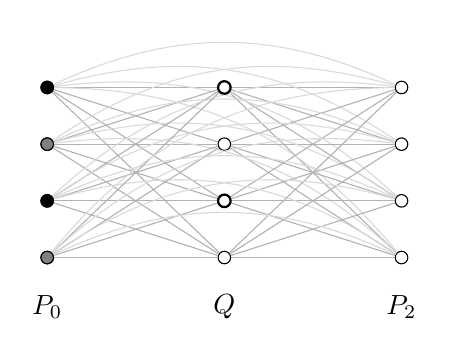
\begin{tikzpicture}[scale=0.9, every node/.style={circle, draw, inner sep=1.6pt}]
\node (a1) at (0,1.2) {}; \node (a2) at (0,0.4) {}; \node (a3) at (0,-0.4) {}; \node (a4) at (0,-1.2) {};
\node (b1) at (2.5,1.2) {}; \node (b2) at (2.5,0.4) {}; \node (b3) at (2.5,-0.4) {}; \node (b4) at (2.5,-1.2) {};
\node (c1) at (5,1.2) {}; \node (c2) at (5,0.4) {}; \node (c3) at (5,-0.4) {}; \node (c4) at (5,-1.2) {};
\foreach \i in {1,2,3,4} \foreach \j in {1,2,3,4} { \draw[gray!60] (a\i) -- (b\j); \draw[gray!60] (b\i) -- (c\j); \draw[gray!30, bend left=25] (a\i) to (c\j); }
\node[fill=black] at (0,1.2) {}; \node[fill=black] at (0,-0.4) {};
\node[fill=gray] at (0,0.4) {}; \node[fill=gray] at (0,-1.2) {};
\node[fill=white, thick] at (2.5,1.2) {}; \node[fill=white, thick] at (2.5,-0.4) {};
\node[draw=none, rectangle] at (0,-1.9) {$P_0$}; \node[draw=none, rectangle] at (2.5,-1.9) {$Q$}; \node[draw=none, rectangle] at (5,-1.9) {$P_2$};
\end{tikzpicture}
\caption{$M_3$ with $n=4$. A pair $\bar d$ in $P_0$ (black), its image $g\bar d$ under a permutation of $P_0$ (grey) and its image $\varepsilon\bar d$ under the transposition $(P_0\,Q)$ (white). Every coherent relation between $\bar d$ and $g\bar d$ witnessed in $M_k$ is also witnessed between $\bar d$ and $\varepsilon\bar d$, since positive atoms only ask for distinct parts.}
\end{figure}

\begin{rem}[compactness]\label{rem:compact}
For each $k\ge1$ the coherent formula
\[
E_k(x,y)\;:=\;x=y\ \vee\ \exists z_1\dots z_{k-1}\Big(\bigwedge_{j}
\big(R(x,z_j)\wedge R(y,z_j)\big)\wedge\bigwedge_{j<l}R(z_j,z_l)\Big)
\]
is an equivalence relation in $T$: in a model with $k'$ parts, $x$ and
$y$ have $k-1$ pairwise adjacent common neighbours iff $k-1$ parts other
than theirs exist, so $E_k$ is equality if $k'<k$, the relation ``same
part'' if $k'=k$ and total if $k'>k$. Hence $\sigma/E_k$ is a coherent
imaginary which agrees with $\Pi$ on the $k$-partite models, and the
object $[\text{exactly $k$ parts}]\times\sigma/E_k$ of $\BB\PP\cC_T$
agrees with $\Pi$ on the $k$-partite models and is empty elsewhere.
The theorem says that no single object of $\BB\PP\cC_T$ agrees with
$\Pi$ on all models, not even on all models with finitely many parts
(the theory also has models with infinitely many parts, on which every
sentence ``exactly $k$ parts'' fails while $\Pi$ is nonempty): the
number of witnesses $k-1$ is unbounded, and a single coherent
equivalence relation, with $w$ witnesses, cannot see the parts of a
$k$-partite model for $k>2m+w+2$. The obstruction is the same
compactness that makes the sharp object of \cite[Thm.~5.6]{TheoryComp}
unreachable in three Morita steps.
\end{rem}

\begin{cor}[lengths of the alternation]\label{cor:length}
For every coherent $\cC$ the alternation starting with the completion
stops after three steps, $\PP\BB\PP\cC\simeq\PP\BB\cC$, and the one
starting with the translation after two. The three steps are needed for
the theory of complete multipartite graphs, and two suffice for Boolean
and for propositional theories.
\end{cor}
\begin{proof}
Proposition~\ref{prop:PB}, Theorem~\ref{thm:order} and
Proposition~\ref{prop:positive}.
\end{proof}

\begin{equation*}
\begin{tikzcd}[column sep=large]
\cC \arrow[r, "\eta_\BB"] \arrow[d, "\eta_\PP"'] & \BB\cC \arrow[r, "\eta_\PP"] & \PP\BB\cC \\
\PP\cC \arrow[r, "\eta_\BB"'] & \BB\PP\cC \arrow[r, "\eta_\PP"'] & \PP\BB\PP\cC \arrow[u, "\simeq"']
\end{tikzcd}
\end{equation*}
The upper row reaches the join in two steps; in the lower row the last
unit is not an equivalence for the theory of Theorem~\ref{thm:order}.

\begin{rem}
Lemma~\ref{lem:full} places the question in classical model theory:
$\BB\PP\cC_T\simeq\PP\BB\cC_T$ iff the Morleyization $T^m$ eliminates
imaginaries relative to the coherent imaginaries of $T$, that is, iff
every $T^m$-definable equivalence relation on a coherent imaginary has
a quotient among the classical subobjects of coherent imaginaries.
Theorem~\ref{thm:order} is a failure of this relative elimination, by a
compactness argument; Proposition~\ref{prop:positive} is its success for
propositional theories, where imaginaries are coproducts of
subterminals.
\end{rem}

\section{Further translations}\label{sec:outlook}

The reading of this paper applies to any translation which is a
reflector, or more generally a $2$-functor, on a $2$-category of
theories, and the three questions it answers for the Morleyization are
to be asked for each: the join with the Morita sameness and its
alternation length; the category of models that detects the join; the
commutation with the completions $\FF$, $\EE$, $\PP$.
\begin{enumerate}
\item The double negation translation on Heyting categories (theories
in intuitionistic first-order logic), $\cC\mapsto$ the Boolean
category of $\neg\neg$-stable subobjects, the coherent objects of
$\Sh_{\neg\neg}$ of the classifying topos: is it a reflector onto Boolean
categories, how does its class compare with $V_\BB$ on the coherent
fragment, and does it commute with $\PP$?
\item The G\"odel--McKinsey--Tarski translation, which reads a Heyting
category as the fixed points of a nucleus on a Boolean algebra object;
the joins of nuclei and their alternation lengths are the subject of
\cite{Fijoin}, and the question is whether a translation of this kind
is a point of the lattice of samenesses or only of a lattice of nuclei.
\item Maruyama's Lawvere--Tierney topologies on syntactic
hyperdoctrines as translations \cite[\S4.10]{Maruyama16}: for an
idempotent $j$, $\rho_j(T)=\{\varphi: T\vdash j\varphi\}$ is a closure
operator on theories, and the question is which $j$ commute with the
Morita completion, Theorem~\ref{thm:order} being the negative answer for
$j=$ Morleyization.
\end{enumerate}

\section*{Declarations}
The author has no competing interests to declare.

\begin{thebibliography}{99}
\bibitem{BH16} T.~W.~Barrett, H.~Halvorson, \emph{Morita equivalence},
Rev. Symb. Log. 9 (2016), 556--582.
\bibitem{CV98} A.~Carboni, E.~M.~Vitale, \emph{Regular and exact
completions}, J. Pure Appl. Algebra 125 (1998), 79--116.
\bibitem{Harnik11} V.~Harnik, \emph{Model theory vs. categorical logic:
two approaches to pretopos completion (a.k.a. $T^{\mathrm{eq}}$)}, in:
Models, Logics, and Higher-Dimensional Categories, CRM Proc. Lecture
Notes 53, Amer. Math. Soc., 2011, 79--106.
\bibitem{Hudetz19} L.~Hudetz, \emph{Definable categorical equivalence},
Philos. Sci. 86 (2019), 47--75.
\bibitem{Elephant} P.~T.~Johnstone, \emph{Sketches of an Elephant: A Topos
Theory Compendium}, Oxford Univ. Press, 2002.
\bibitem{LV01} S.~Lack, E.~M.~Vitale, \emph{When do completion processes
give rise to extensive categories?}, J. Pure Appl. Algebra 159 (2001),
203--230.
\bibitem{MR77} M.~Makkai, G.~E.~Reyes, \emph{First Order Categorical
Logic}, Lecture Notes in Math. 611, Springer, 1977.
\bibitem{Maruyama16} Y.~Maruyama, \emph{Meaning and Duality: From
Categorical Logic to Quantum Physics}, D.Phil. thesis, University of
Oxford, 2016.
\bibitem{Same} R.~Shibusawa, \emph{The sameness lattice of a category:
weak-equivalence structures, Galois functoriality, and comparison intervals},
preprint (2026), archived at DOI 10.5281/zenodo.22823772.
\bibitem{Fijoin} R.~Shibusawa, \emph{Joins of localisations in the lattice of
two-out-of-three classes: the finite-iteration criterion for closure
operators on exact categories, with applications to toposes, torsion
theories and fuzzy sets}, preprint (2026), archived at DOI
10.5281/zenodo.23691896.
\bibitem{TheoryComp} R.~Shibusawa, \emph{Comparing theories in the lattice
of two-out-of-three classes: Morita equivalence as a join of completions,
the forced order of coproducts and quotients, and conceptual completeness
as an identity of samenesses}, preprint (2026), archived at DOI
10.5281/zenodo.24095158.
\bibitem{Tsem17} D.~Tsementzis, \emph{A syntactic characterization of
Morita equivalence}, J. Symbolic Logic 82 (2017), 1181--1198.
\end{thebibliography}

\end{document}
